\documentclass[11pt, oneside]{article} 
\usepackage{geometry}
\geometry{letterpaper} 
\usepackage{graphicx}
	
\usepackage{amssymb}
\usepackage{amsmath}
\usepackage{parskip}
\usepackage{color}
\usepackage{hyperref}

\graphicspath{{/Users/telliott_admin/Tex/png/}}
% \begin{center} 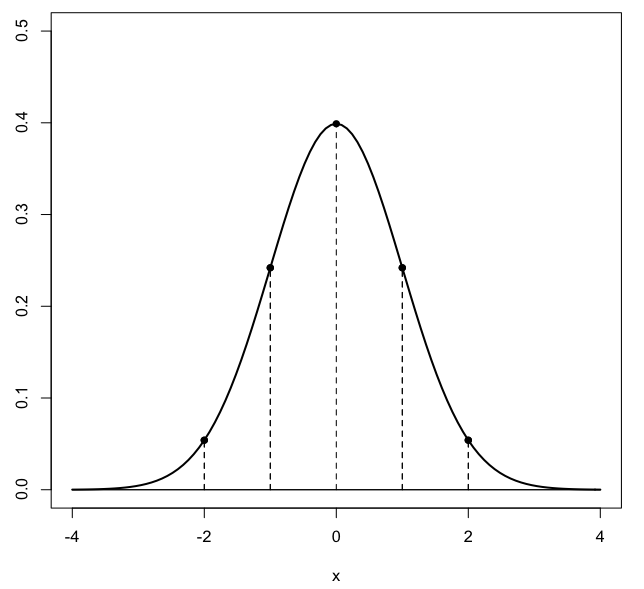
\includegraphics [scale=0.4] {gauss3.png} \end{center}

\title{problem}
\date{}

\begin{document}
\maketitle
\Large

Suppose we are given two points on the graph of a parabola.  Can we find the equation of the parabola?

Let the two points be $(2,3)$ and $(4,8)$.  The general equation for a parabola oriented vertically is
\[ y = ax^2 + bx + c \]
so
\[ 3 = 4a + 2b + c \]
\[ 8 = 16a + 4b + c \]
We have three unknowns but only two equations.

There is something else, however.  Quadrature says that the slope of the chord is equal to the slope of the curve at the midpoint of the chord.  The slope of the chord is $5/2$.

The midpoint is at $x=3$.  The slope there is $2ax + b = 6a + b$ so
\[ 5/2 = 6a + b \]
Eliminate $c$ from the first pair of equations
\[ 5 = 12a + 2b \]
These are not independent so we have no help.








\end{document}